%\documentclass[aps,prstab,showpac,twocolumn]{revtex4-1}  
%\documentclass[aps,prstab,onecolumn,preprint]{revtex4-1}
\documentclass[aps,prstab,onecolumn,preprint,endfloats,11pt]{revtex4-1}

\usepackage{graphicx}
\usepackage{epsfig}
\usepackage{subfigure}
\usepackage{fancyhdr}
\usepackage{color}
\usepackage{amsfonts}
\usepackage{amsmath}
\usepackage{amssymb}
\usepackage{dcolumn}
\usepackage{bm}
\usepackage{indentfirst}
\usepackage{rotating}
\usepackage{moreverb}


\linespread{1.0}

\makeatletter

\begin{document}

\title{Studies of Particle Motions During Slow Resonant Extraction}
\author{Chong Shik Park, James Amundson, Leo Michelotti, and Vladimir Nagaslaev}
\affiliation{Fermi National Accelerator Laboratory, PO Box 500, Batavia, IL 60510}
\date{\today}

\begin{abstract}
We present beam dynamics simulation studies for third-integer resonant extraction at Fermi Mu2e experiment. Dynamic bumps are implemented for local orbit corrections in which septum entrance angle is controlled to reduce angular spread of extracted beams. We perform particle tracking simulations to investigate arrival time profile of extracted particles as well as distributions of scattered particles. We also discuss motions of particles with RFKO beam heating, which will help to understand spill regulations using RFKO feedback system.
\end{abstract}

\pacs{}
\maketitle

\setcounter{tocdepth}{7}

%\tableofcontents

\section{\label{sec:intro}Introduction}

For the Mu2e experiment at Fermilab, the slow resonant extraction method provides proton pulses from the Delivery Ring to the production target system~\cite{tdr}. Using the accelerator simulation package, Synergia2, we have performed resonant extraction simulations, and results are discussed in~\cite{mu2e}. The main goal of beam dynamics simulations is to demonstrate third-integer resonant extraction of proton beams with stable spill structure. The third-integer resonance is excited with the harmonic sextupoles, and slow spills are generalized by ramp tune-qaud strengths. 
Talbe~\ref{table:param} shows beam and machine parameters we have used in this paper for the Mu2e resonant extraction simulations. 

To meet the extraction beam requirements, we adopt a pice-wise ramp profile, septum plane rotaions, and RFKO feedback system, described in the reference~\cite{mu2e}. 

\begin{table*}[!bp]
 %\begin{center}
    \begin{tabular}{rrr}
    \hline
     Parameters                & Value              & Units         \\
    \hline
      Beam Momentum     & 8.886    & GeV/c   \\
      Beam Intensity/Spill         &  1 & Tp ($10^{12}$ protons)       \\
      $B \rho$                  & 29.650             & T-m           \\
      Bunch Length (rms)        & 40                 & nsec          \\
      95 \% invariant normalized emittance & 20     & $\pi$ mm-mrad \\
      Ring Circumference  & 505.283            & m             \\
      Resonant Tune($\nu_{x})$   & 29/3 &  \\
      Bare Tunes, ($\nu_{x0}$, $\nu_{y0}$)   & (9.65, 9.78)   &    \\
      Momentum Spread ($\Delta p / p$)       & 0.0016         &    \\
      Spill Duration &  54  & msec \\
      $N_{\text{turn}} / {\text{spill}}$    & 31,795   &    \\
      Protons per pulse     & 31.5  &  Mp ($10^{6}$ protons)  \\
      Harmonic Number           & 4                  &               \\
      RF Frequency              & 2.36               & MHz           \\
      RF Peak Voltage                & 10                 & kV            \\
    \hline
    \end{tabular}
    \caption{\label{table:param}Beam and Machine Parameters}
  %\end{center}
\end{table*}

Sec.~\ref{sec:bump} discusses local orbit corrections with dynamic bumps. In Sec.~\ref{sec:tracking}, arrival time profile measurements and scattered particle tracking simulations are presented using Synergia2. Tracking simulations with analytical equations of motion using the Kobayshi Hamiltonian method are also compared. Sec.~\ref{sec:rfko} describes particles' motions under the influence of RFKO beam heating.


\clearpage
\section{\label{sec:bump}Local Orbit Corrections with Dynamic Bumps}

\subsection{\label{sec:bump0}Septum Entrance Angle}

In the previous paper~\cite{mu2e}, we discussed that a septum foil plane should be aligned with particles' entrance angles to the septum.
This alignment of the septum foil plane should be optimized in the manner of reducing particle losses due to crossing the plane from outside to inside a septum field region or vice versa.
In the Delivery Ring, however, the septum is placed at a zero dispersion section, and all shrinking separatrices are always centered at origin during extraction.
These yield that the Hardt condition, a condition to arrange separatrix geometries by superimposing them for different momenta, cannot be fulfilled~\cite{pullia}.
Consequently, particles' angle coordinates at the entrance of the first septum are not aligned with a fixed septum foil plane.

\begin{figure*}[!tbp]
  \subfigure[Before applying dynamic bumps]{
    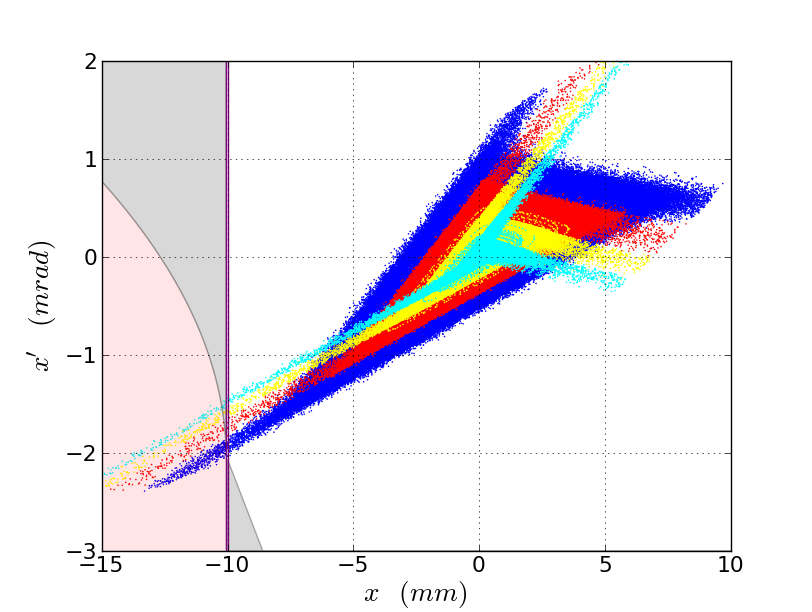
\includegraphics[width=.45\textwidth]{img/fig_bump1a.png}
    \label{fig:bump00}}
  \subfigure[After applying dynamic bumps]{
    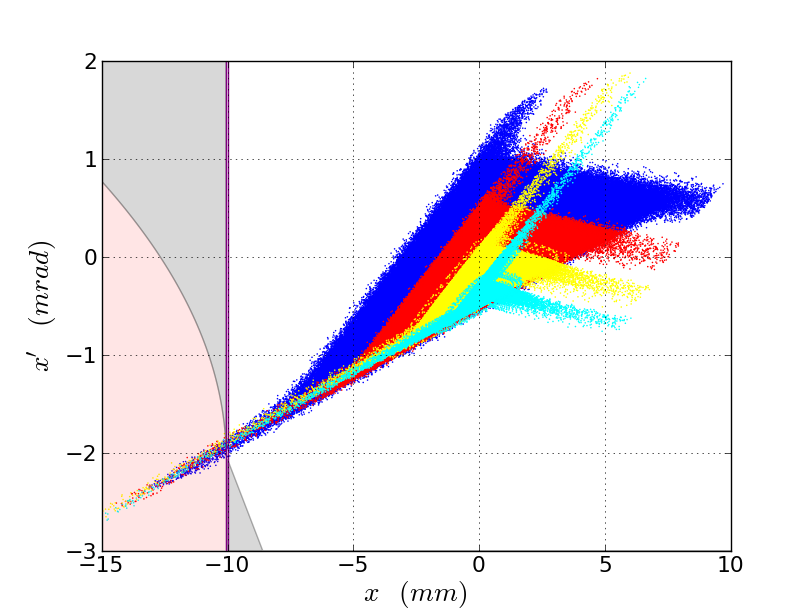
\includegraphics[width=.45\textwidth]{img/fig_bump1b.png}
    \label{fig:bump01}}
  \caption{\label{fig:bump0}Phase space plots of particles for 4 different extraction stages (turns 100(blue), 6000(red), 20000(yellow), and 30000(cyan)): (a) before and (b) after applying dynamic bump corrections. (Color: Red shaded part is the septum field region, and gray shaded one is the septum shadow regions.)}
\end{figure*}

Fig.~\ref{fig:bump00} shows a phase space of particles for four different extraction stages (turns 100, 6,000, 20,000, and 30,000).
As separatrix is squeezed by increasing tune-quad strengths, unstable particles are streamed along branches of separatrices. 
The septum field region (color: red shaded) is formed on the [left] side of the vertical septum foil line (color: purple) at $x=10$~mm. 
Gray shaded regions on the plot are defined as septum shadow regions in which particles will be considered as lost.
%The detailed explanation of the septum shadow regions is in Appendix~\ref{sec:shadow}.
Streams of unstable particles on the [leftmost] separatrix branch for each extraction stage are entering the septum field region by crossing the septum foil line.
However, their entering angles are moving [upward] during the extraction processes.
An angle of the septum foil plane is aligned with an initial extraction stage.
, the alignment is only valid for few turns at the beginning, and there will be continuous misalignment of the septum foil plane later.
These result that more particles are entering the [upper] septum shadow region (color:gray shaded), and they will be lost eventually.
Variations of angle coordinates at the septum entrance will be seen at the experiment target with a large horizontal angular spread of extracted beams.

In our case with the septum at a zero dispersion section, two possible ways can be considered to have same entrance angles of particles to the septum for different extraction stages.
The first method is to compensate the beam angle by rotating separatrices. This could be achievable by changing phases of two harmonic sextupole circuits.
The phase contributions of each harmonic circuit differs by about 90 deg, and these make phase adjustments doable.
However, particles' entrance angles for different extraction stages are same only if their $x$ coordinates are equal to the horizontal position of the septum foil at the entrance, $x_{ES}$.
In other words, their angles beyond $x_{ES}$ will be diverged.
These yield an asymmetric angular spread of extracted beams.

The other solution is to apply local orbit corrections using angle bumps throughout the spill.
Extracted particles will have a symmetric angular spread during the spill as well as same entrance angles.
For resonant extraction from the Delivery ring, we chose a local orbit correction scheme.
Particles' orbits in the extraction beamline will be dynamically corrected with four bump magnets.
As a backup solution to prepare a failure of local bump corrections, the harmonics sextupole magnets and their power supplies are designed to preserve ramp capabilities.
In this paper, we will only discuss how local bump corrections are implemented, and detailed specifications for magnets and power supplies are presented in the Mu2e TDR~\cite{tdr}.

\subsection{\label{sec:bump1}Dynamic Bumps}

\begin{figure}[!tbp]
  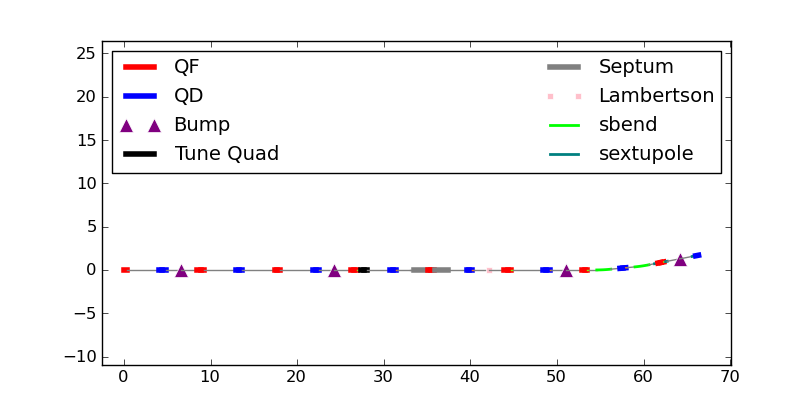
\includegraphics[width=.45\textwidth]{img/fig_bump2}
  \caption{\label{fig:bump1}Schematic drawing of the external beamline with four local orbit bumps.}
\end{figure}

Using four dynamic bumps, we could align separatrices to reduce angular deviations at the entrance of the septum.
Fig.~\ref{fig:bump1} is a schematic drawing of four dynamic bump locations in the extraction beamline.
Two bumps are located at the upstream of septa, and the other two are at the downstream.
Upstream bumps kick particles so that bases of separatrices are aligned during an entire extraction period.
Then, downstream bumps will kick them back to original orbits.
Fig.~\ref{fig:bump01} presents a phase space plot of particles for different extraction stages after applying local orbit corrections.
All triangular distributions of particles are well aligned on their bases.
The [leftmost] branch arms are extended to the same direction, i.e., particles are entering the septum field region with same angular extensions.

Strengths of local orbit corrections can be easily obtained by applying a transfer matrix method with initial closed orbit conditions.
With the condition that the closed orbit is zero outside bumps, their strengths in time, $\theta_{i}(t)$ for $i=1,2,3,4$, are given by
\begin{equation}
  \begin{split}
  \theta_{1}(t) & = - \sqrt{\frac{\beta_{s}}{\beta_{1}}}
               \frac{\sin(\psi_{s} - \psi_{2})}
                    {\sin(\psi_{2} - \psi_{1})}
               \Delta x_{s}^{\prime} (t),
  \\ %\;\;\;
  \theta_{2}(t) & = \sqrt{\frac{\beta_{s}}{\beta_{2}}}
               \frac{\sin(\psi_{s} - \psi_{1})}
                    {\sin(\psi_{2} - \psi_{1})}
               \Delta x_{s}^{\prime} (t), \\
  \theta_{3}(t) & = \sqrt{\frac{\beta_{s}}{\beta_{3}}}
               \frac{\sin(\psi_{s} - \psi_{4})}
                    {\sin(\psi_{4} - \psi_{3})}
               \Delta x_{s}^{\prime} (t),
  \\ %\;\;\;\;\;\;\;\;\;\;
  \theta_{4}(t) & = - \sqrt{\frac{\beta_{s}}{\beta_{4}}}
               \frac{\sin(\psi_{s} - \psi_{3})}
                    {\sin(\psi_{4} - \psi_{3})}
               \Delta x_{s}^{\prime} (t),
  \end{split}
  \label{eqn:bump}
\end{equation}
where $\beta_{i}$'s are betatron functions at septum($s$) and bumps($1,2,3,4$), $\psi_{i}$'s are betatron phase advances, and $\Delta x^{\prime}_{s} (t)$ is required angle kick of particles at the septum entrance as a function of time.
Fig.~\ref{fig:bump2} shows changes of bump strengths vs.~time.
Since particles' entrance angles to the septum are aligned to the initial extraction stage, bump strengths are zero at the beginning and are maximum at the end of extraction.
From Eq.(~\ref{eqn:bump}), we observed that strengths of bump magnets would be getting smaller, when the distance of each pair for upstream and downstream bumps are closer.
Since each magnet is bounded between two quadrupoles, there are limitations in minimizing their strengths.

\begin{figure}[!tbp]
  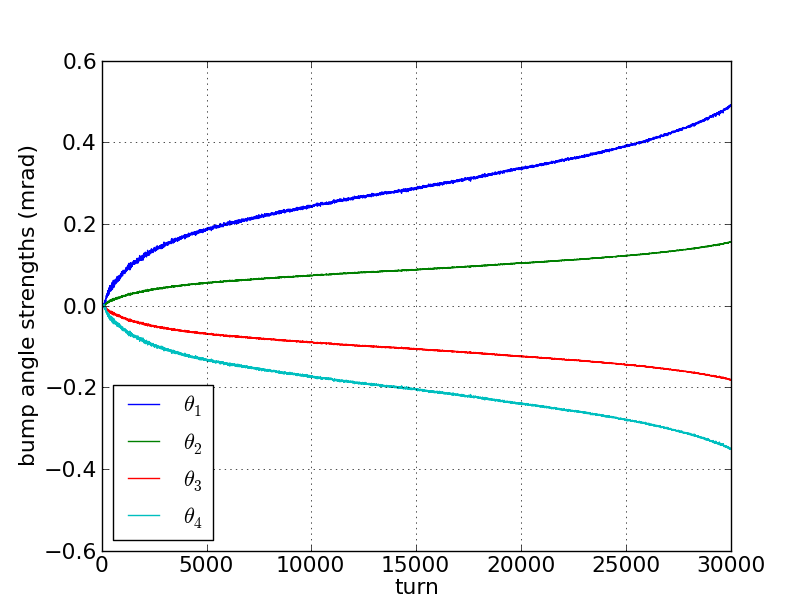
\includegraphics[width=.45\textwidth]{img/fig_bump3}
  \caption{\label{fig:bump2}Strengths changes of dynamic bumps in time.}
\end{figure}

\subsection{\label{sec:bump2}Simulation Results}

In Fig.~\ref{fig:bump3}, footprints of extracted particles at the entrance of the first septum are plotted in phase space coordinates.
These are accumulations of extracted particles with and without local orbit corrections throughout entire extraction period.
Particles (color: blue) survived from lost or scattered by the septum element will be transferred to the 2nd septum, a Lambertson magnet, and a C-magnet.
They will be then extracted to the external beamline.
Particles (color: black) formed a thin line on the [right] hit the septum foil with 50$\mu$m at the entrance during spill.
Some particles (color: red) intersect the septum foil plane by entering the septum shadow region (color: gray shaded).
The last two kinds of particles are removed and considered as lost in simulations.
The horizontal phase space ellipses (color: green), which match the beam with 99.9\% containment, are plotted alongside.

Before applying local orbit corrections, the footprint has a wider angular spread and there are many beam losses due to crossing the foil plane as seen in Fig.~\ref{fig:bump30}.
However, Fig.~\ref{fig:bump31} shows a narrower angular thickness of the extracted particle distribution with dynamic orbit corrections.
The footprint of the extracted beam without dynamic bumps is matched to an unnormalized emittance of [1.26]~$\pi$~mm-mrad and its matching horizontal betatron function is [9.1]~m. The local orbit corrected beam has a [0.55]~$\pi$~mm-mrad emittance and [20.1]~m betatron function.
After applying local orbit corrections, angular spreads of the beam also depend on the tune spread as the separatrix is squeezed.
The Delivery Ring has a nonzero chromaticity for the sufficient mixing of the coherent RFKO excitation~\cite{ipac11}.
Therefore, a chromatic tune spread causes a little spread of angle coordinates as seen in Fig.~\ref{fig:bump31}, while the overall emittance of the corrected beam is smaller compared to that of uncorrected beam.

\begin{figure*}[!tbp]
  \subfigure[Before applying dynamic bumps]{
    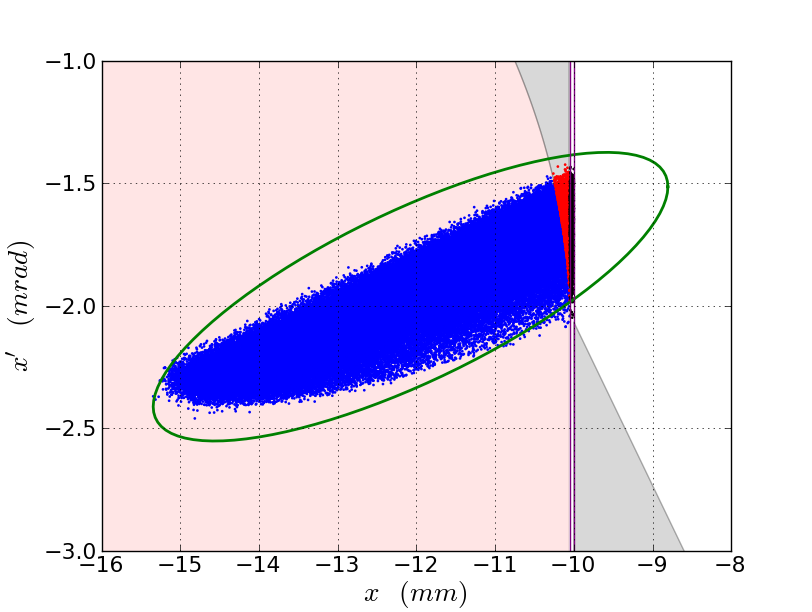
\includegraphics[width=.45\textwidth]{img/fig_bump4a}
    \label{fig:bump30}}
  \subfigure[After applying dynamic bumps]{
    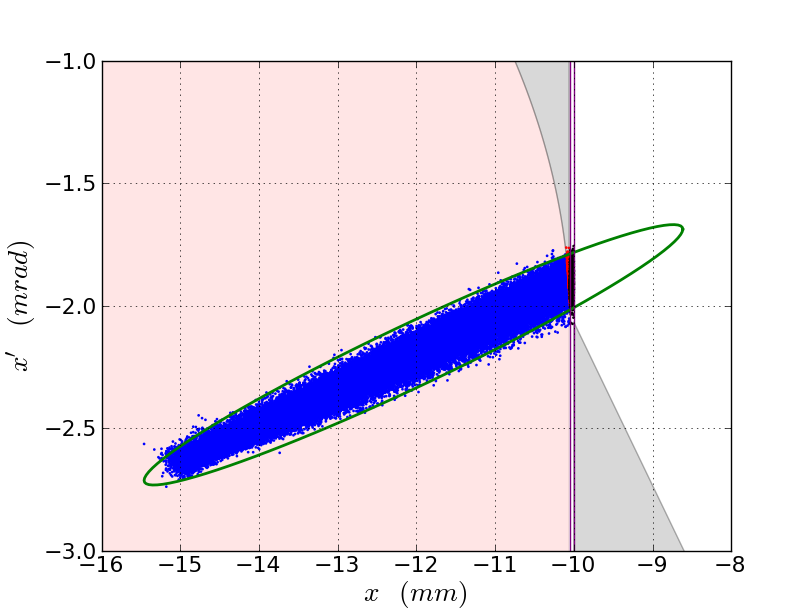
\includegraphics[width=.45\textwidth]{img/fig_bump4b}
    \label{fig:bump31}}
  \caption{\label{fig:bump3}Footprints of extracted particles with and without dynamic bumps. (Color: Blue dots are to-be-extracted particles, red dots are lost particles by intersecting the septum foil plane, and black dots are lost particles by hitting the septum. Red shaded part is the septum field region, and gray shaded one is the septum shadow regions.)}
\end{figure*}

As described in the previous paper~\cite{mu2e}, Synergia2 has a septum aperture to detect particle losses by hitting a septum head or crossing a septum foil plane.
The rotation of the septum plane is taken into account in the model.
Fig.~\ref{fig:bump4} shows extraction simulation results of particle losses with and without local orbit corrections during the spill.
While ``hit\_septum1'' and ``hit\_septum2'' are losses by hitting entrances of septum elements, ``cross\_septum1'' and ``cross\_septum2'' are losses by crossing septum foil planes for the 1st and 2nd septa, respectively.
``total\_losses'' are a sum of turn-by-turn particle losses for each turn.

Without dynamic angle corrections, septum planes are aligned only to the beginning of the extraction stage.
Therefore, beam losses are rising in time due to mismatching of the alignment (see Fig.~\ref{fig:bump40}).
When dynamic bumps correct beam orbits, particles' entrance angles are well matched to septum foil planes.
In Fig~\ref{fig:bump41}, turn-by-turn particle losses are not changing much and are much smaller compared with no orbit corrections.
We also observed that losses at the 2nd septum with dynamic bumps are decreased.

\begin{figure*}[!tbp]
  \subfigure[Before applying dynamic bumps]{
    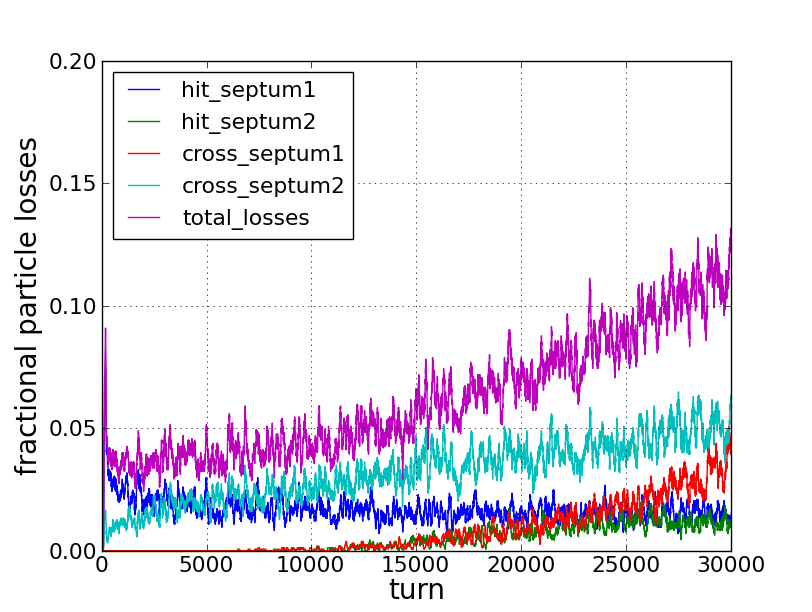
\includegraphics[width=.45\textwidth]{img/fig_bump5a}
    \label{fig:bump40}}
  \subfigure[After applying dynamic bumps]{
    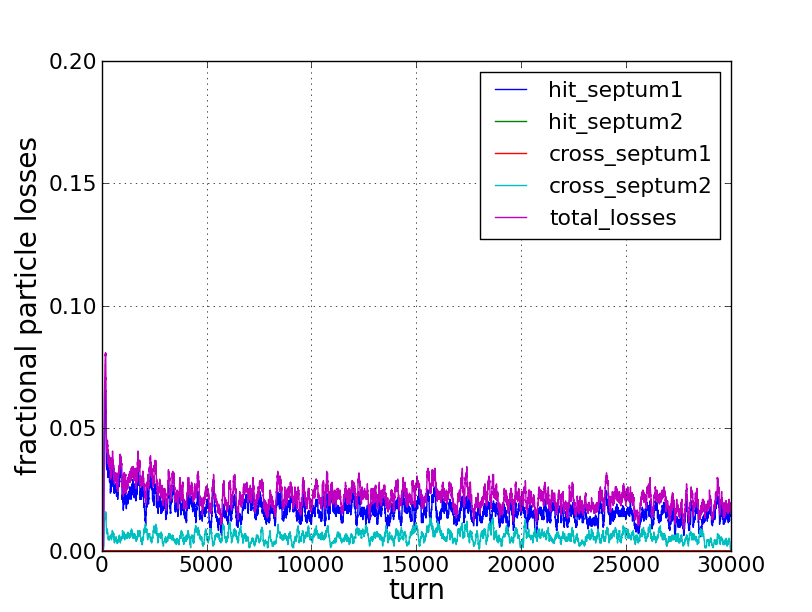
\includegraphics[width=.45\textwidth]{img/fig_bump5b}
    \label{fig:bump41}}
  \caption{\label{fig:bump4}Particle losses in time with and without dynamic bumps.}
\end{figure*}

%%%%%%%%%%%%%%%%%%%%%%%%%%%%%%%%%%%%%%%%%%%%%%%%%%%%%%%%%%%%%%%%%%%%%%%%%%%

\section{\label{sec:tracking}Particle Tracking Simulations}

\subsection{\label{sec:model}Simplified Resonance Model and Kobayashi Hamiltonian}

With a complex, normalized, horizontal phasespace coordinates, $a = [x + i (\alpha x + \beta x^{\prime})] / \sqrt{2 \beta}$, the Hamiltonian for the third-integer resonance model based on the perturbation theory can be derived as~\cite{preliminary}
\begin{equation}
  H = \Delta \nu \cdot a^{*} a - i g a^{3} + i g^{*} a^{*} + \cdots,
\label{eqn:hamiltonian1}
\end{equation}
where $\Delta \nu$ is the difference between the horizontal and resonant tunes, and $g$ is  a linear functional of the sextupole field strength distribution:
\begin{equation*}
  g = \frac{i}{6 \sqrt{2}} \frac{1}{4 \pi} \sum_{\text{sextupoles}}
      \Bigg[
        \frac{B^{\prime\prime} l}{(B\rho)} \beta^{3/2}
        e^{-i 3(\psi - \Delta \nu \theta)}
      \Bigg].
\end{equation*}
By changing variables to real, normalized coordinates, $(X, X^{\prime}) = (x/\sqrt{\beta}, (\alpha x + \beta x^{\prime}) / \sqrt{\beta})$, in Eq.~(\ref{eqn:hamiltonian1}), with $g = |g| e^{i \Psi}$, the Hamiltonian has the new form,
\begin{widetext}
\begin{equation}
  H = \frac{\Delta \nu}{2} \left( X^{2} + X^{\prime2} \right)
    + \frac{|g|}{\sqrt{2}}
      \Big[
        \left( X^{3} - 3 X X^{\prime 2} \right) \sin{\Psi}
      + \left( 3 X^{2} X^{\prime} - X^{\prime 3} \right) \cos{\Psi}
      \Big].
\label{eqn:hamiltonian2}
\end{equation}
\end{widetext}
The orientation of the separatrix at the entrance of the first septum is formed an upright triangle in the normalized phase space by setting $\Psi = \pi$. With multiplying by $6 \pi$ to Eq.~(\ref{eqn:hamiltonian2}), a well-known Kobayashi Hamiltonian can be obtained
\begin{equation}
  H_{K} = \frac{\epsilon}{2} \left( X^{2} + X^{\prime2} \right)
    + \frac{S}{4} \left( 3 X^{2} X^{\prime} - X^{\prime 3} \right),
\label{eqn:kobayashi}
\end{equation}
where $\epsilon = 6\pi \Delta \nu$, and a normalized sextupole strength, $S = 12\sqrt{2} \pi |g| \cdot \text{sgn}(\Delta \nu)$. 

The Kobayashi Hamiltonian describes motions of particles in the phase space coordinates for every three turn~\cite{kobayashi}.
The first term of $H_{K}$ prescribes the unperturbed linear motion of particles, and their motions are described as circles in the normalized phase space. For Mu2e resonant extraction, $\Delta \nu = \nu_{x} - 29/3$, thus the machine tune is set to below resonance. This yields that particles inside the separatrix are rotating counterclockwise direction. The second term contributes the perturbed motion of particles associated with harmonic sextupoles. Due to this term, stable particles are bounded by the triangular separatrix, while unstable particles are streaming away along the outgoing separatrix branches. 
% discussions about the Kobayashi Hamiltonian can be found in references~\cite{pullia}.

With Eq.~(\ref{eqn:kobayashi}), equations of motion are given by
\begin{equation}
 \begin{split}
  \frac{dX}{dt} & = \frac{\partial H_{K}}{\partial X^{\prime}}
                  = \epsilon X^{\prime} + \frac{3}{4} S
                    \left(
                      X^{2} - X^{\prime 2}
                    \right), \\
  \frac{dX^{\prime}}{dt} & = - \frac{\partial H_{K}}{\partial X}
                           = - \epsilon X - \frac{3}{2} S X X^{\prime}.
%   \frac{dX}{dt} & = \frac{\partial H_{K}}{\partial X^{\prime}}
%                   = \frac{3}{4} S
%                     \left(
%                       X^{2} + \frac{4}{3} \frac{\epsilon}{S} X^{\prime}
%                     - X^{\prime 2}
%                     \right), \\
%   \frac{dX^{\prime}}{dt} & = - \frac{\partial H_{K}}{\partial X}
%                            = - \frac{3}{2} S \left( X^{\prime}
%                             + \frac{2}{3} \frac{\epsilon}{S} \right) X.
 \end{split}
\label{eqn:motion}
\end{equation}
The unit of the time in Eq.~(\ref{eqn:motion}) is three consecutive turns, i.e., $t = 1 [\times 3 \; \text{turns}] = 3 T_{\text{rev}}$[sec], where $T_{\text{rev}} \simeq 1.6 \mu$sec.
Compared to the total spill time (54 msec), three turns (3 $\times$ 1.6 $\mu$sec) can be considered as an infinitesimal time increment, therefore the particle motion is adiabatic. 

Using the simplified resonance model described above and accelerator simulation package, Synergia2, we measure arrival time of particles streaming to the septum plane, perform tracking simulations for particles scattered by septum foils.


\subsection{\label{sec:arrival}Arrival Time Profile}

For the slow resonant extraction methods, one of the most important parts is to maintain stable spills during the entire extraction. With the help of optimal tune-ramp profile and RFKO feedback system, multi-particle tracking simulations using Synergia2 showed \mbox{$\pm 20\%$} variations in spill structures~\cite{mu2e}. However, it is quite possible to have unwanted spill fluctuations in the presences of magnet imperfections or magnet power supply ripples. Moreover, the RFKO feedback system to regulate the spill rate for the Mu2e experiment requires precise predictions of those fluctuations. 

In this section, we will discuss arrival time profiles of extracted particles using Synergia2 tracking simulations. An arrival time is defined as a transition time change of a particle from the unstable region to the septum field region. This is called as the transit time in the reference~\cite{pullia}. As M. Pullia suggested, the arrival time profile of extracted particles could help to predict and provide behaviors of spill structures under influences of magnetic field variations.

Analytical expressions for the arrival time(transit time) in the reference \cite{pullia} were derived based on equations of motion from the Kobayashi Hamiltonian. With these formulas, the transit times were given for either a constant resonance or a slowly varying resonance. However, we realized that it is hard to predict arrival time with approximations used in~\cite{pullia}, especially when particles are close to stable fixed points. Particles' motions are strongly bounded near the stable fixed points, and it takes longer time to escape these points, and therefore, the transit time calculated with analytical expressions easily goes infinity.

\begin{figure*}[!tbp]
  \subfigure[Beam intensities]{
    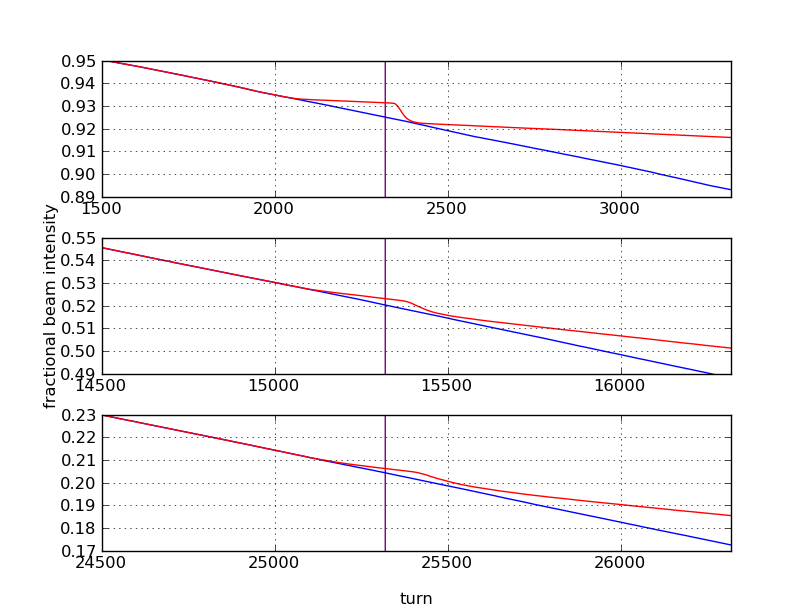
\includegraphics[width=.45\textwidth]{img/fig_arrival1a}
    \label{fig:arrival11}}
  \subfigure[Particles' $x$ coordinates and their distribution vs. arrival time]{
    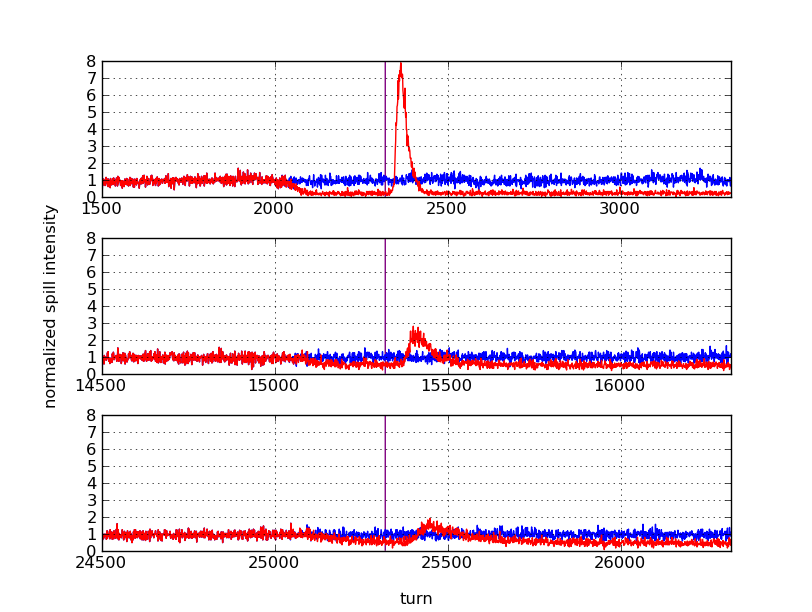
\includegraphics[width=.45\textwidth]{img/fig_arrival1b}
    \label{fig:arrival12}}
  \caption{\label{fig:arrival1}Arrival Time Measurement Stages. (top:early, middle:middle, and bottom:end}
\end{figure*}

Synergia2 tracking simulations are prepared to measure arrival times for extracted particles. 500k macro particles are initially injected and slowly extracted in the Delivery Ring. Other beam and machine parameters are listed in Table[\textcolor{red}{table reference}] The optimal tune-quads ramp profile provides a constant slow spill. At a selected turn, tune-quads ramp are intentionally stopped, and their strengths are kept constant for about $\sim$1\% of the spill duration, roughly $\sim$300 turns. During this first constant ramp period, a small amount of beam could be extracted. After this period, strengths of tune-quads are restored to original settings instantaneously and kept constant again. The second constant period is for about \textcolor{red}{500/1000} turns, which should be enough to observe whole transitions of unstable particles to the septum field region. During the transition, the amount of affected particles are relatively small, so that particles inside the narrow separatrix shell induced by the tune jump are involved, and we measure arrival times for those particle transitions. 

As the separatrix is shrinking by the tune ramp, its distance to the septum field region is getting longer. Therefore, the arrival time depends on the extraction stage, and we choose three different stages for measurement points: early ($\sim$2000 turn), middle ($\sim$15,000 turn), and close to the end ($\sim$25,000 turn). 500k macro particles in the initial beam is large enough to observe a smooth transition distribution for each stage.

Fig.~\ref{fig:arrival11} shows quadrupole strengths vs.~turn for three different stages (top:early, middle:middle, and bottom:end). \textcolor{red}{Dashed} lines (color:blue) are beam intensities with a normal ramp profile, while solid lines (color:red) are those with paused ramp profiles explained above. Each solid line shows small extraction rates during first constant ramp periods, and there are sudden drops of beam intensities after passing restored tune points, shown with vertical lines (color:purple). The turn-by-turn normalized beam intensities are shown in Fig.~\ref{fig:arrival12}. Ideal normalized intensities should be 1.0, and spill intensities with normal ramp profile are close to the ideal one. With a paused ramp profile for the arrival time measurements, spill intensities are reduced during constant ramp periods. Since sizes of separatrices are relatively small in last two stages, thicknesses of separatrix changes induced by tune variations are very thin, therefore we observe that spill intensities are not reduced as much in the early stage. For the early stage, this separatrix change is large enough to hold many unstable particles inside the separatrix, so that extracted particle rates are very small during the constant ramp and there are large bursts of particles after restoring. 

\begin{figure*}[!tbp]
  \subfigure[Turn 2,000]{
    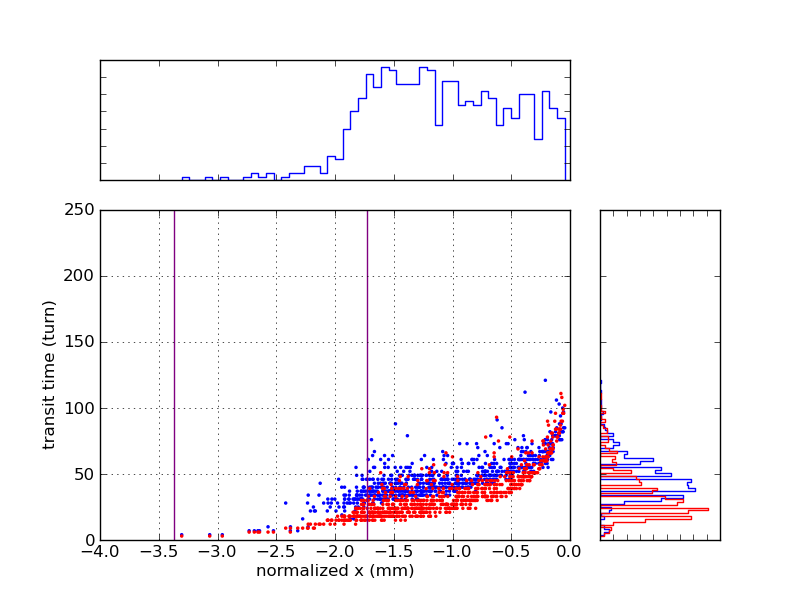
\includegraphics[width=.3\textwidth]{img/fig_arrival2a}
    \label{fig:arrival21}}
  \subfigure[Turn 15,000]{
    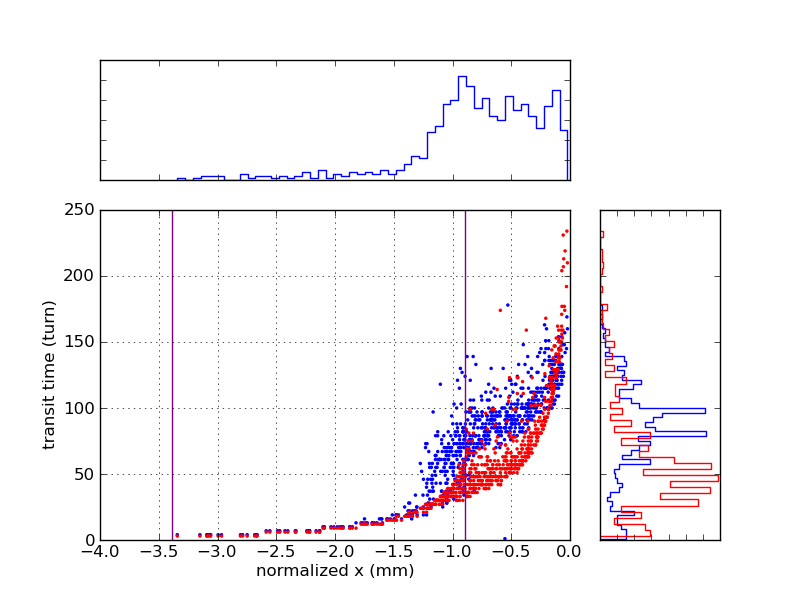
\includegraphics[width=.3\textwidth]{img/fig_arrival2b}
    \label{fig:arrival22}}
  \subfigure[Turn 25,000]{
    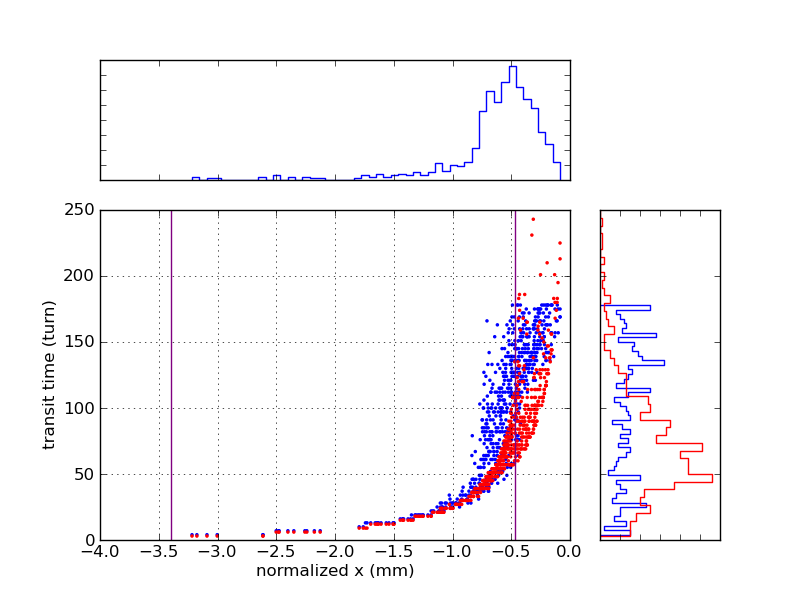
\includegraphics[width=.3\textwidth]{img/fig_arrival2c}
    \label{fig:arrival23}}
  \caption{\label{fig:arrival2}Arrival Time Distributions. (left:early, middle:middle, and right:end)}
\end{figure*}

Besides Synergia2 tracking simulations, we also track particles' motions with the Kobayashi Hamiltonian method to calculate arrival times. By solving equations of the motion in Eq.~(\ref{eqn:motion}) with 4th order Runge-Kutta (RK4) method, particle's motions are tracked for every three-turn and their arrival times are calculated. For the one-to-one comparison, their initial positions are set same as those of Synergia2 tracking simulations, however, space charge effects are excluded for simplicity reasons. Effective normalized sextupole strengths are calculated with harmonic sextupole strengths at the second tune stopping points.

In Fig.~\ref{fig:arrival2}, arrival time profiles of particles are plotted as a function of their initial positions. Each dot represents an individual particles with Synergia2 (\textcolor{red}{triangle}, blue) and RK4 (\textcolor{red}{circle}, red) methods. Attached plots on top and right are histograms of their distributions. The left vertical line is the septum foil position, and the right one indicates the $x$ coordinates of the leftmost unstable fixed point. 

When particles are sitting on or slightly off the outgoing separatrix branch, arrival times are almost same for two methods. However, there are large offsets between two methods, if particles' initial positions are near the side of the separatrix triangle. Speed of the transit time varies particles' distance from the separatrix line. In other words, the arrival time is inversely proportional to the distance between particle and separatrix. This is predicted in M.~Pullia's analytical expressions, too. In the RK4 method, we also exclude space charge effects, which shake particle's motions and eventually varies distance to the separatrix. Consequently, these effects make particles travel more time to reach the septum field region. Moreover, both cases have relatively large arrival times near the unstable fixed point, shown with large peaks in the upper histogram plots. Since particles starting near this point are strongly bounded by restoring forces, escape times are longer than other initial positions. 


\subsection{\label{sec:beamloss}Beam Loss Tracking}

In slow resonant extraction, unstable particles outside the separatrix are separated from the circulating beam and streaming through the separatrix branches. When these particles are entering the septum field region, they are kicked by electrostatic fields biased between septum foils and cathode. For the Mu2e experiment, two septa are placed with 50~$\mu$m thickness foils. Due to the finite thickness and width of foils, some particles have chances to hit these foils and scatter throughout the beamline. In order to reduce these hitting rates, we adopt many techniques. such as septum foil plane rotation, dynamic bumps, and diffusers. Synergia2 tracking studies predicted that these chances are approximately less than 2\%. 

Synergia2 has capability of filtering these particles at the entrance of the septum, and handles as beam losses. That is, it does not track scattered particles inside and after septum elements. In the real machine, particles could cross a gap between two foils, or be scattered by foils. If these particles go back into the field free region, they will circulate with the existing circulating beam, again. In case of entering into the septum field region, they will be partially kicked by the electrostatic fields. Of these scattered particles, some could be survived by scattering, however, most of them will hit a beam pipe somewhere around the ring and generate very hazardous radio-activities.

In order to observe behaviors of scattered particles, we use the MARS code in conjunction with Synergia2~\cite{mars1}. MARS is a Monte Carlo code with capabilities of hardronic and electromagnetic cascades for particles in accelerators, detectors, spacecrafts, etc~\cite{mars2}. Fig.~\ref{fig:beamloss1} shows a beam tracking with the MARS code through the extraction channel in the Delivery Ring. The extraction channel consists of two electrostatic septa (ESS1 and ESS2), a Lambertson magnet (ELAM), and two quadrupoles (Q203 and Q204). Two main streams with black traces representing protons are circulating (upper) and outgoing (lower) particles. Outgoing particles will be transported to the C-magnet and extracted. Other colored traces are secondary particles scattered by the septum foils. Circulating and outgoing beams are separated in the first septum, ESS1. At ESS2, their separation is large enough to have no losses. 

\begin{figure*}[!tbp]
  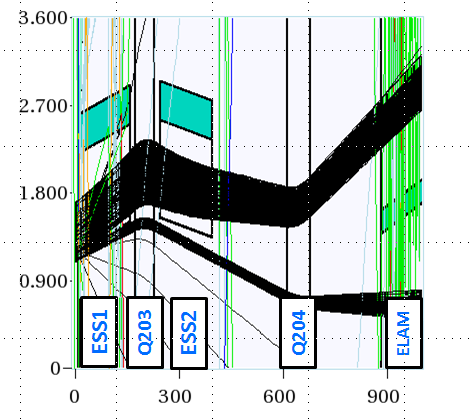
\includegraphics[width=3.2in]{img/fig_beamloss1}
  \caption{\label{fig:beamloss1} Plan view for the MARS tracking in the extraction channel. Main lattice elements are marked with labels. Only extracted beam and a small fraction of the circulating beam are shown. Black traces show protons, secondary particles are shown in other colors.}
\end{figure*}

In Synergia2 multi-particle tracking simulations, a specialized aperture at the entrance of the first septum is applied to filter out lost particles. This aperture consists of two parts: 1) determine particle hittings to the first foil head or other septum components at its entrance, and 2) calculate particle trajectories inside the septum to check their crossings over the septum plane. After applying the septum aperture, the collection of filtered particles are prepared as an input of MARS tracking simulations. In MARS simulations, filtered particles are tracked through the extraction channel from the first septum (ESS1) to the C-magnet. Each septum has detailed geometries of foil configurations, such as foil thickness, width, separations, material properties, etc. Therefore, particles cascade motions can be tracked in detail. Then, the second Synergia2 tracking simulations perform with scattered particles from the MARS output starting at the C-magnet. 

\begin{figure*}[!tbp]
  \subfigure[Synergia2 Tracking Results]{
    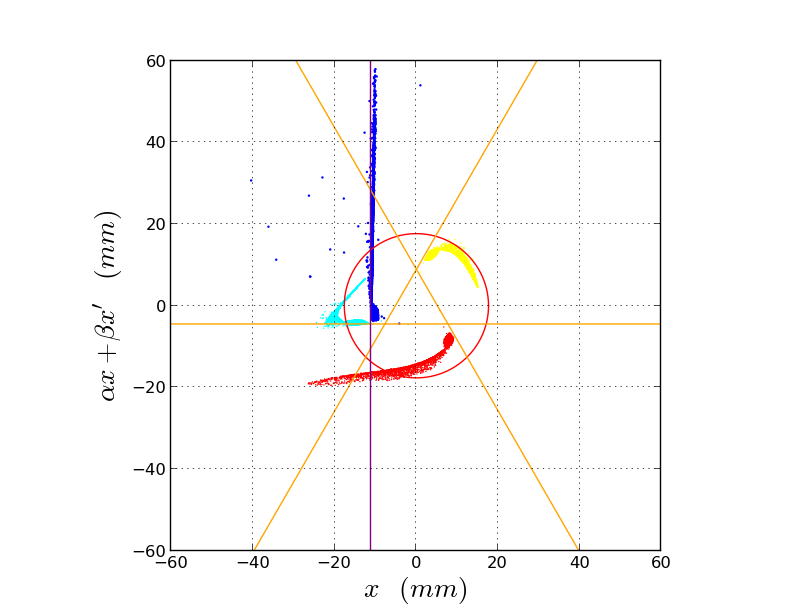
\includegraphics[width=.45\textwidth]{img/fig_beamloss2a}
    \label{fig:beamloss21}}
  \subfigure[Beam loss locations]{
    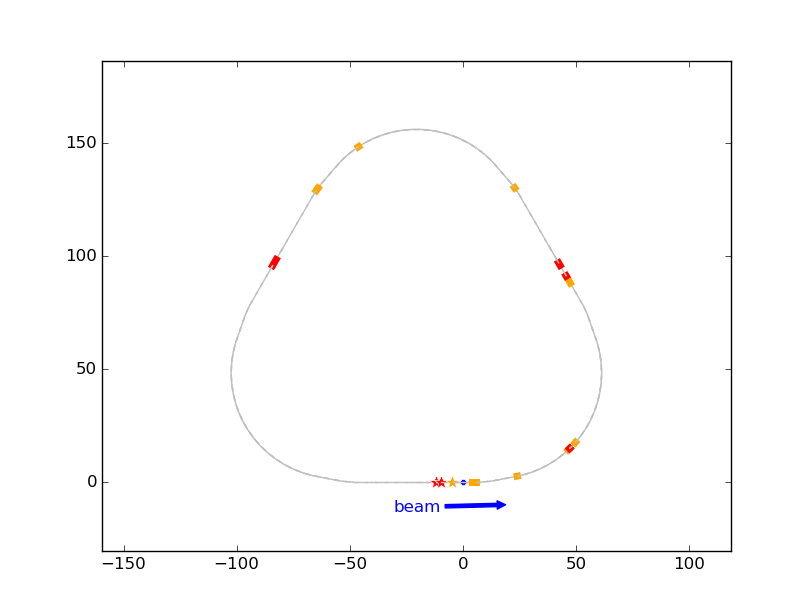
\includegraphics[width=.45\textwidth]{img/fig_beamloss2b}
    \label{fig:beamloss22}}
  \caption{\label{fig:beamloss2}Synergia2 tracking results for scattered particles at the entrance of the first septum: a) turn-by-turn results with normalized phasespace coordinates, b) beam loss locations.}
\end{figure*}

Fig.~\ref{fig:beamloss21} shows turn-by-turn tracking results for scattered particles at the entrance of the first septum in normalized phasespace coordinates. Particles (color:blue) along with the vertical line (color:purple) at 11~mm are input sample particles from MARS results. Their original measured locations are at the C-magnet, but we traced them back to the septum just for the comparison. We also add arbitrary circulating particles, which are shown as a large block at one edge of their distribution. Particles after 1, 2, and 3 revolutions are plotted on the bottom, right, and left, respectively. After 3 turns, most of survived particles are inside the septum field region. Fig.~\ref{fig:beamloss22} shows where scattered particles are lost inside the ring. Black line represents the beamline of the Delivery Ring. This plot shows that beam losses are occurred mostly at septa elements, first arc section, and middles of each straight section. From simulations results, about \~43\% particles are lost, while the rest of particles are survived and extracted. 

In Fig.~\ref{fig:beamloss21}, we observe that distributions of scattering particles have curved shapes after each revolution, although its initial distribution is well aligned along the line. After the third revolution, it has V-like shape distribution in which particles along the outgoing separatrix branch are our additional circulating particles, not scattered particles. That is, scattered particles are off from the separatrix branch. To examine these behaviors, we use equations of motion with the Kobayashi Hamiltonian, again. Particles' motions are tracked for every 3 turns using Eq.~(\ref{eqn:motion}), and those are plotted in Fig~\ref{fig:beamloss3}. In this tracking simulation, there are no extraction channel including septa and Lambertson, so that there is no extraction. Particles (color:blue) aligned with the septum line (vertical line) are initial particle distributions (turn 0). The Flipped S-like shape distribution (color:red) is at the next third turn, and the remaining distribution is the final 6th turn. Although all initial particles are aligned on the straight line at the beginning, they are sitting on the different field line. In other words, they are moving with different speeds along the distinguished hyperbola trajectories. 


\begin{figure*}[!tbp]
  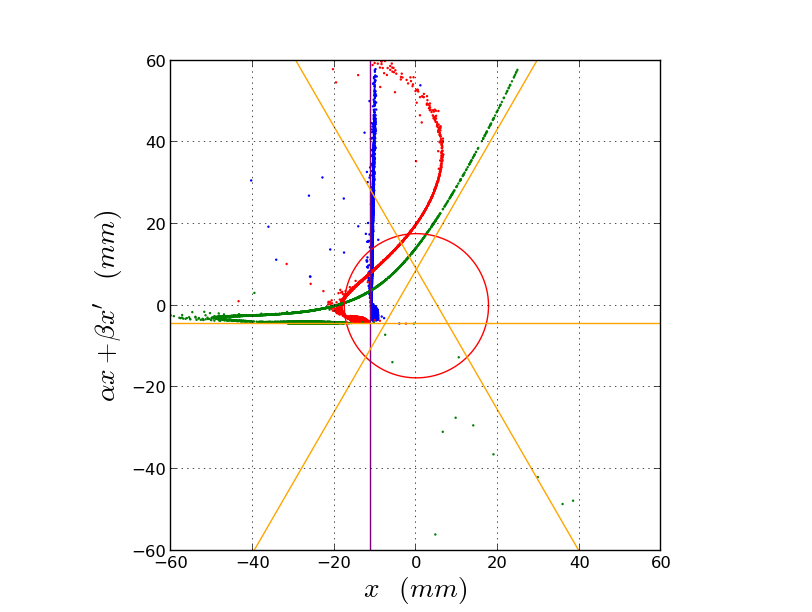
\includegraphics[width=3.2in]{img/fig_beamloss3}
  \caption{\label{fig:beamloss3} RK4 tracking results.}
\end{figure*}


\clearpage
\section{\label{sec:rfko}Particle Motions with RFKO Beam Heating}

\subsection{\label{sec:dist}Beam Distribution Function}

\subsection{\label{sec:emit}Emittance Growth Rates}

\section{\label{sec:conclusion}Conclusion}

\section{\label{thanks}Acknowledgments}

This work was supported by the United States Department of Energy under contract DE-AC02-07CH11359 and the ComPASS project funded through the Scientific Discovery through Advanced Computing program in the DOE Office of High Energy Physics.

% \appendix
% \section{\label{sec:shadow}The Septum Shadow Region}
% \subsection{Outside the Septum Field Region}
% \subsection{Inside the Septum Field Region}

\begin{thebibliography}{77}
 %%\documentclass[aps,prstab,showpac,twocolumn]{revtex4-1}  
\documentclass[aps,prstab,onecolumn,preprint,nofootinbib]{revtex4-1}

\usepackage{graphicx}
\usepackage{epsfig}
\usepackage{subfigure}
\usepackage{fancyhdr}
\usepackage{color}
\usepackage{amsfonts}
\usepackage{amsmath}
\usepackage{amssymb}
\usepackage{dcolumn}
\usepackage{bm}
\usepackage{indentfirst}
\usepackage{rotating}
\usepackage{moreverb}

\setlength{\textwidth}{6.5in}
\setlength{\textheight}{8.5in}
\setlength{\topmargin}{0in}
\setlength{\oddsidemargin}{0.0in}
\setlength{\evensidemargin}{0.0in}
\setlength{\rightmargin}{0.0in}

\makeatletter

\begin{document}

\title{Studies of Particle Motions During Slow Resonant Extraction}
\author{Chong Shik Park, James Amundson, Leo Michelotti, and Vladimir Nagaslaev}
\affiliation{Fermi National Accelerator Laboratory, PO Box 500, Batavia, IL 60510}
\date{\today}

\begin{abstract}
We present here 
%The Mu2e experiment at Fermilab requires the acceleration and transport of intense proton beams, and the delivery of stable and uniform particle spills to the production target. To meet the experimental requirement, particles will be slowly extracted from the Delivery Ring to the external beamline. Using Synergia2, we have performed multi-particle tracking simulations of the third-integer resonant extraction in the Delivery Ring, including space charge effects as well as physical beamline elements and apertures. With a suitable ramp profile of tune-quadrupoles, we modeled a uniform spill structure. In order to minimize beam losses which are critical for efficient extractions, we have implemented a number of features, such as apertures in beamline elements, septum plane alignments. The RF Knockout (RFKO) technique, which excites particles transversely, is employed as a spill regulation system. Combined with a feedback system, it assists in fine-tuning the spill uniformity. Simulation studies have been carried out to optimize the RFKO feedback scheme, which will be helpful in designing the spill regulation system. 
\end{abstract}

\pacs{}
\maketitle

\setcounter{tocdepth}{5}

%\tableofcontents

%%%%%%%%%%%%%%%%%%%%%%%%%%%%%%%%%%%%%%%%%%%%%%%%%%%%%%%%%%%%%%%%%%%%%%
\section{\label{sec:intro}Introduction}

\clearpage
\section{\label{sec:bump}Phasespace Corrections with Dynamic Bumps}

In the previous paper, we discussed that a septum foil plane should be aligned with particles' $x^{\prime}$ coordinates when they are entering the field region of the septum. This alignment of the septum foil plane alogn with $x^{\prime}$s should be optimized to reduce particle losses due to crossing the plane from outside to inside the field region or vice versa. However, particles' angle coordinates are changing in time when a separatrix is being squeezed during an extraction period. 
Fig.~\ref{fig:bump0} shows unstable particles measured at the entrance of the first septum in normalized phase space coordinates for 4 different stages of extraction. Particle streams are entering the septum field region by crossing the vertical line (color:purple), and their coordinates are changing during the extraction.
Therefore, the alignment is only valid for a few turns at the beginning, and there will be misalignments of the septum foil plane with respect to $x^{\prime}$s later. These result in increasing of beam losses in time. Moreover, one can expect that an angular spread of extracted particles at the entrance of the septum will be large.

\begin{figure*}[tbh!]
  \begin{center}
    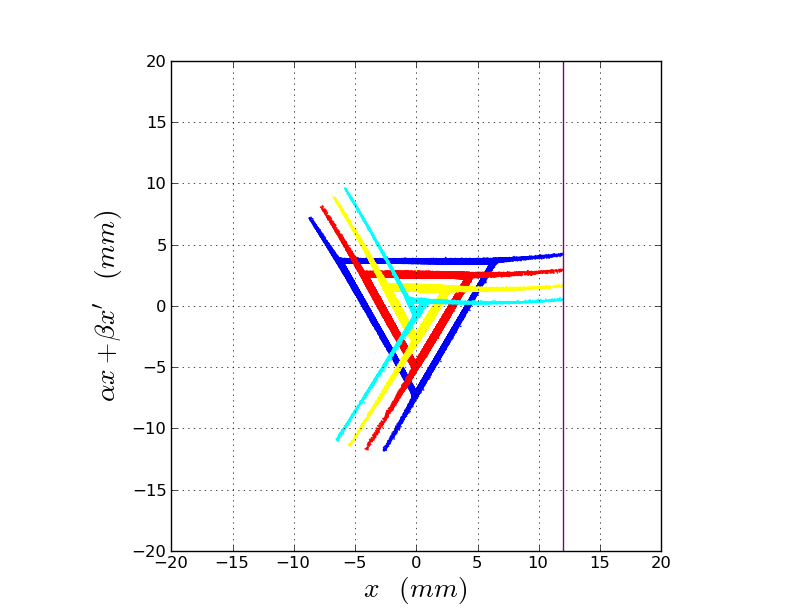
\includegraphics[width=.45\textwidth]{img/ufp.png}
    \caption{\label{fig:bump0}Normalized phase space plots of particles around separatrices.}
  \end{center}
\end{figure*}



\begin{figure*}[tbh!]
  \begin{center}
    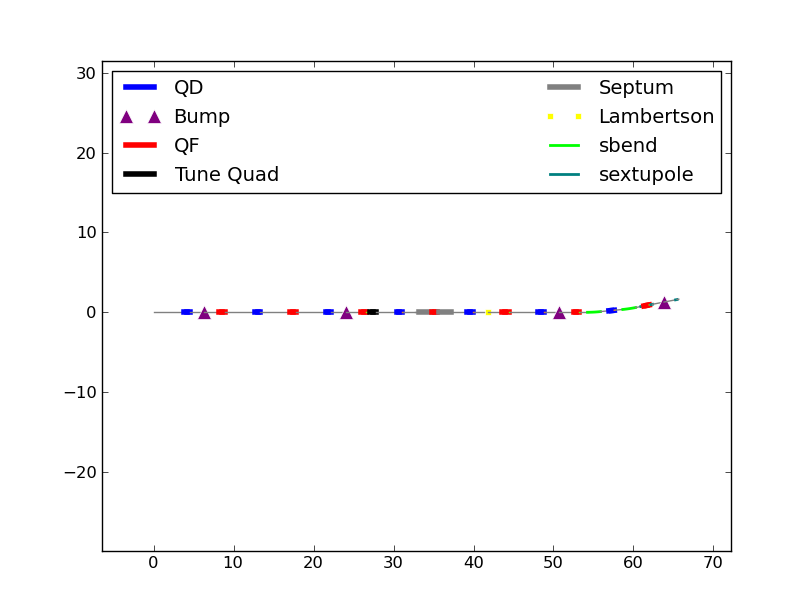
\includegraphics[width=.45\textwidth]{img/20140109-00.png}
    \caption{\label{fig:bump1}Schematic drawing of the external beamline with 4 dynamic bumps.}
  \end{center}
\end{figure*}


In order to mitigate these effects, orbit corrections are applied using 4 dynamic angle bumps. Fig.~\ref{fig:bump1} shows a schematic drawing of 4 dynamic bump locations in the extraction beamline. 2 bumps are located at the upstream of septa, and the other 2 are at the downstream. Upstream bumps kick particles so that outgoing particles' angles are aligned at the entrance end of the first septum during the entire extraction period. Then, downstream bumps will kick them back to original positions.

Using simple Bump strengths, $\theta_{i}$ for $i=1,2,3,4$, are given by
\begin{equation}
  \begin{split}
  \theta_{1}(t) & = \sqrt{\frac{\beta_{s}}{\beta_{1}}}
               \frac{\sin(\psi_{s} - \psi_{2})}
                    {\sin(\psi_{2} - \psi_{1})}
               \left( - \Delta x_{s}^{\prime} (t) \right),
  \;\;\;
  \theta_{2}(t) = \sqrt{\frac{\beta_{s}}{\beta_{2}}}
               \frac{\sin(\psi_{s} - \psi_{1})}
                    {\sin(\psi_{2} - \psi_{1})}
               \Delta x_{s}^{\prime} (t), \\
  \theta_{3}(t) & = \sqrt{\frac{\beta_{s}}{\beta_{3}}}
               \frac{\sin(\psi_{s} - \psi_{4})}
                    {\sin(\psi_{4} - \psi_{3})}
               \Delta x_{s}^{\prime} (t),
  \;\;\;\;\;\;\;\;\;\;
  \theta_{4}(t) = \sqrt{\frac{\beta_{s}}{\beta_{4}}}
               \frac{\sin(\psi_{s} - \psi_{3})}
                    {\sin(\psi_{4} - \psi_{3})}
               \left( - \Delta x_{s}^{\prime} (t) \right),
  \end{split}
\end{equation}
where $\beta_{i}$'s are betatron functions at the septum($s$) and bumps($1,2,3,4$), $\psi_{i}$'s are betatron phase advances, and $\Delta x^{\prime}_{s} (t)$ is required changes of angle coordinates at the septum as a function of time. Fig.~\ref{fig:bump2} shows changes of bump strengths in time. Since particles' angles are aligned to the initial angle, bump strengths are zero at the beginning and are maximum at the end of extraction.

\begin{figure*}[tbh!]
  \begin{center}
    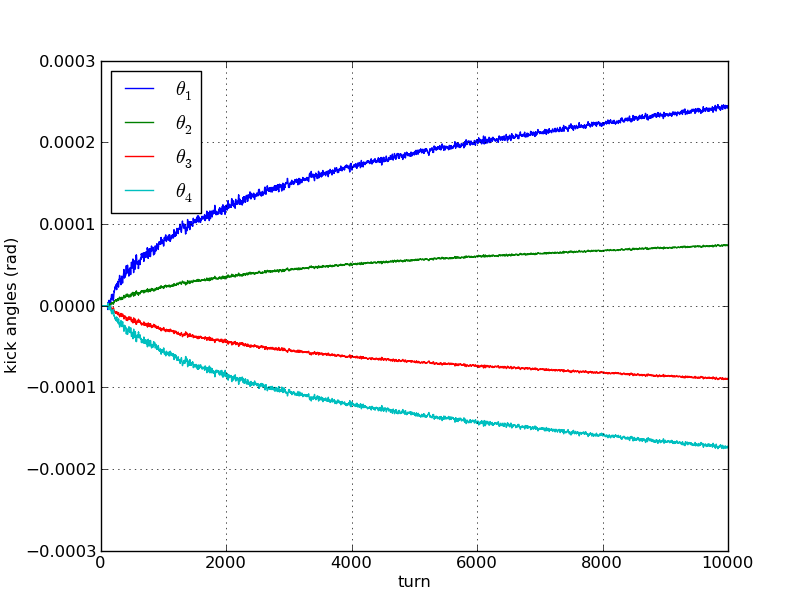
\includegraphics[width=.45\textwidth]{img/20140123-00.png}
    \caption{\label{fig:bump2}Strength changes of dynamic bumps in time.}
  \end{center}
\end{figure*}

Before applying dynamic bumps, phase space of circulating particles are centered at the origin as shown in Fig.~\ref{fig:bump0}. As the separatrix is squeezed by increaing tune-quad strengths, phase space areas are shrinking in time and outgoing branches 


\begin{figure*}[tbh!]
  \begin{center}
    \subfigure[Without Dynamic Bumps]{
      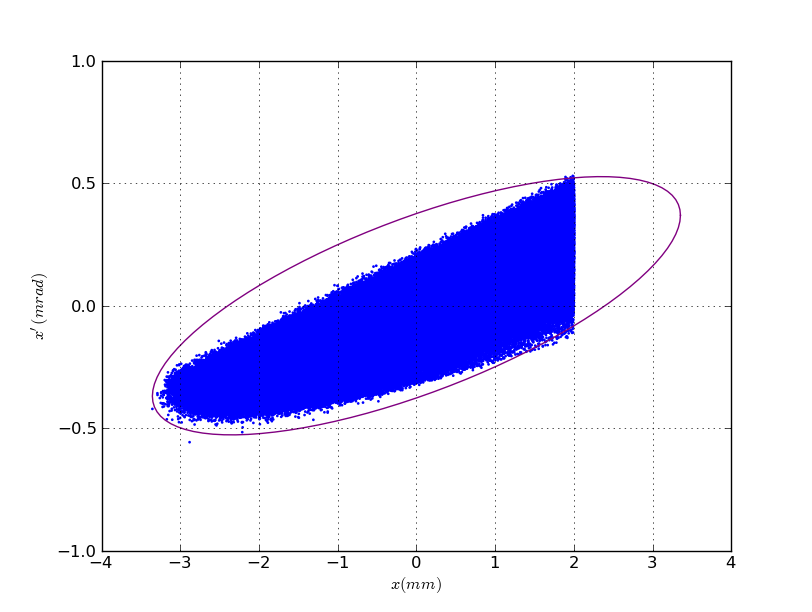
\includegraphics[width=.45\textwidth]{img/20140206-02.png}
      \label{fig:bumpps3}}
    \subfigure[With Dynamic Bumps]{
      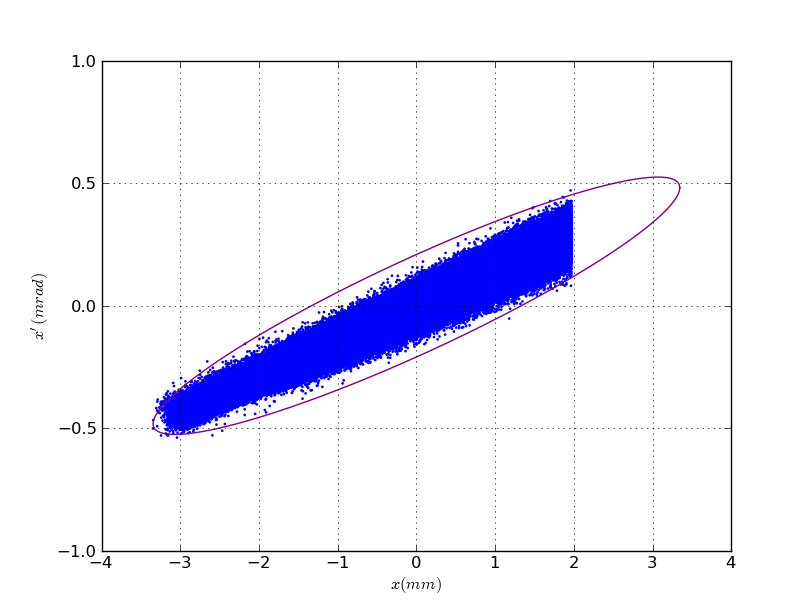
\includegraphics[width=.45\textwidth]{img/20140206-03.png}
      \label{fig:bumpps4}}
    \caption{\label{fig:bump4}Footprints of extracted particles with/without dynamic bumps.}
  \end{center}
\end{figure*}

\begin{figure*}[tbh!]
  \begin{center}
    \subfigure[Without Dynamic Bumps]{
      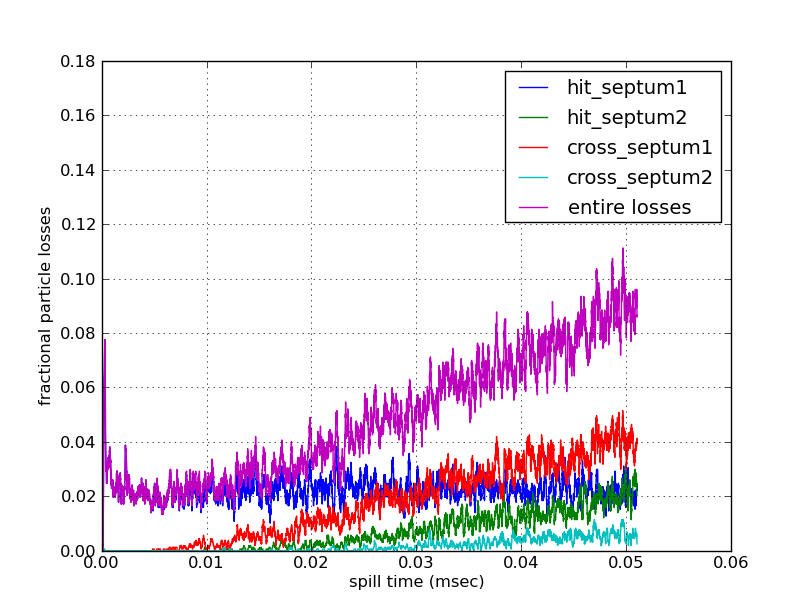
\includegraphics[width=.45\textwidth]{img/20140203-06.png}
      \label{fig:bumploss1}}
    \subfigure[With Dynamic Bumps]{
      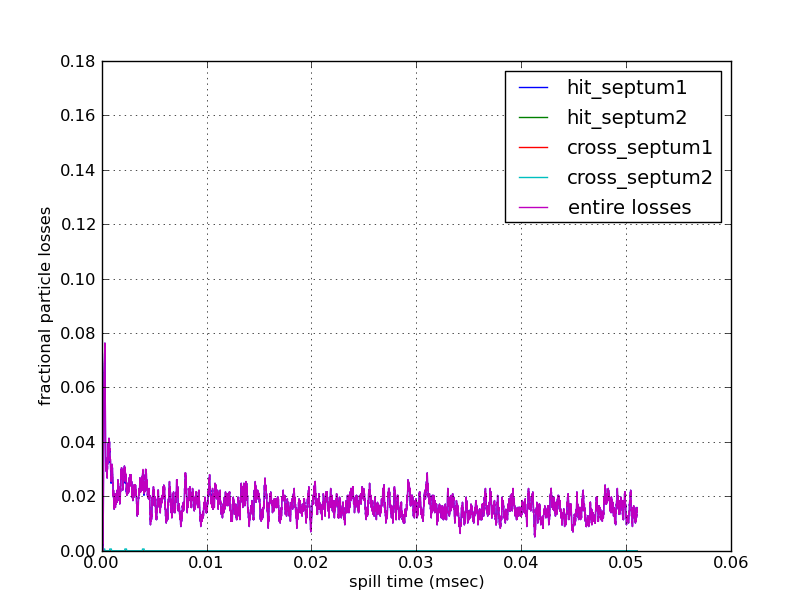
\includegraphics[width=.45\textwidth]{img/20140203-07.png}
      \label{fig:bumploss2}}
    \caption{\label{fig:bump5}Particle losses in time with/without dynamic bumps.}
  \end{center}
\end{figure*}

\section{\label{sec:loss}Tracking of Particle Losses}



\section{\label{sec:emit}Emittance Growth Rates with RFKO Beam Heating}

\section{\label{sec:rfko}RFKO Beam Distribution Function}

\section{\label{sec:arrival}Arrival Time Distribution}

\section{\label{sec:conclusion}Conclusion}

\section{\label{thanks}Acknowledgments}

\begin{thebibliography}{77}


\end{thebibliography}

\end{document}

  \bibitem{tdr}
  Mu2e Technical Design Documentation

  \bibitem{mu2e}
  C.S. Park, ``Tracking Simulation of the Third-Integer Resonant Extraction for the Fermilab Mu2e Experiment,'' submitted to PRST-AB.

  \bibitem{ipac11}
  V. Nagaslaev, J.F. Amundson, J.A. Johnstone, C.S. Park, and S.J. Werkema, 
``Third Integer Resonance Slow Extraction Using RFKO at High Space Charge,'' in 
IPAC 2011 proceeding.

  \bibitem{preliminary}
  L. Michelotti and J. Johnstone, ``Preliminaries Toward Studying Resonant 
Extraction from
the Debuncher,'' Technical Report, Fermilab, 2009. FERMILAB-FN-0842-APC-CD.

  \bibitem{kobayashi}
  Kobayashi paper

  \bibitem{pullia}
  M. Pullia, thesis

  \bibitem{mars1}
  V. Nagaslaev, MARS simulations for Mu2e resonant extraction, in preparation

  \bibitem{mars2}
  N.V. Mokhov, Recent Mars15 developments: nuclide inventory, DPA and gas production ,Fermilab-Conf-10-518-APC (2010)

.
\end{thebibliography}


\end{document}

%sagemathcloud={"zoom_width":100}
